 \section{Results}
\label{sec:results}
In this Section we present some of the results obtained with our planner. The complete sequences computed are shown in the companion video, TODO.
Specifically, we demonstrate the planner for two really different robots, in a large vartiety of environments: the humanoid HRP-2 and the quadriped Hyq.
For each scenario we indicate the heuristics chosen. We also provide a performance analysis, that shows that the planner is compatible with interactive applications,
and present the success rates obtained in each scenario.
We also demonstrate the interest of our robustness criterion in the different computed poses.
Finally, a last example suggests possible applications to dextrous manipulation.

In our ISRR conference paper~\citep{tonneauisrr15}, additional results are demonstrated with various virtual avatars (Figure~\ref{fig:robots_old}).
In this extension we choose to focus on results obtained with actual robots. We invite the interested reader to watch the ISRR video\endnote{https://www.youtube.com/watch?v=LmLAHgGQJGA}, and 
to refer to the previous paper for a discussion on these results.

\begin{figure}[t]
\centering
  \begin{overpic}[width=1\linewidth]{figures/robots_old}
		%~ \put (5,58) {1)} 
		%~ \put (37,58) {2)} 
		%~ \put (68,58) {3.a)} 
		%~ \put (5,27) {3.b)} 
		%~ \put (37,27) {4.a)} 
		%~ \put (68,27) {4.b)} 
	\end{overpic}
\caption{Virtual avatars in various scenarios demonstrated in our conference paper.}
		   \label{fig:robots_old}
\end{figure}

\subsection{Description of the scenarios}
In all the scenarios considered, the formulation of the problem is always the same:
a start and goal root placements are provided as an input of the scenario.
The framework computes the initial contact configuration, and outputs a sequence of contact configurations connecting it to the goal.
In each scenario we detail the parameters chosen: the heuristics, and the constraints on the reachable workspaces (for instance in all the scenarios,
the reachable workspaces of the legs of HRP-2 are always required to intersect with the environment). 
A companion video available at TODO \url{http://youtu.be/LmLAHgGQJGA} (anonymous link) displays the complete contact sequence obtained in all these scenarios.

% \subsubsection*{Truck egress (Figure~\ref{res_truck_pres} and Figure~\ref{res_truck_bd}) -- Humanoid and insectoid robots.}
%\subsubsection*{Truck egress -- Humanoid and insectoid robots (Figure~\ref{res_truck_bd}).}
\subsubsection{HRP-2 -- Steep staircase (Figure~\ref{fig:standing}):}

\begin{figure*}
  \centering
  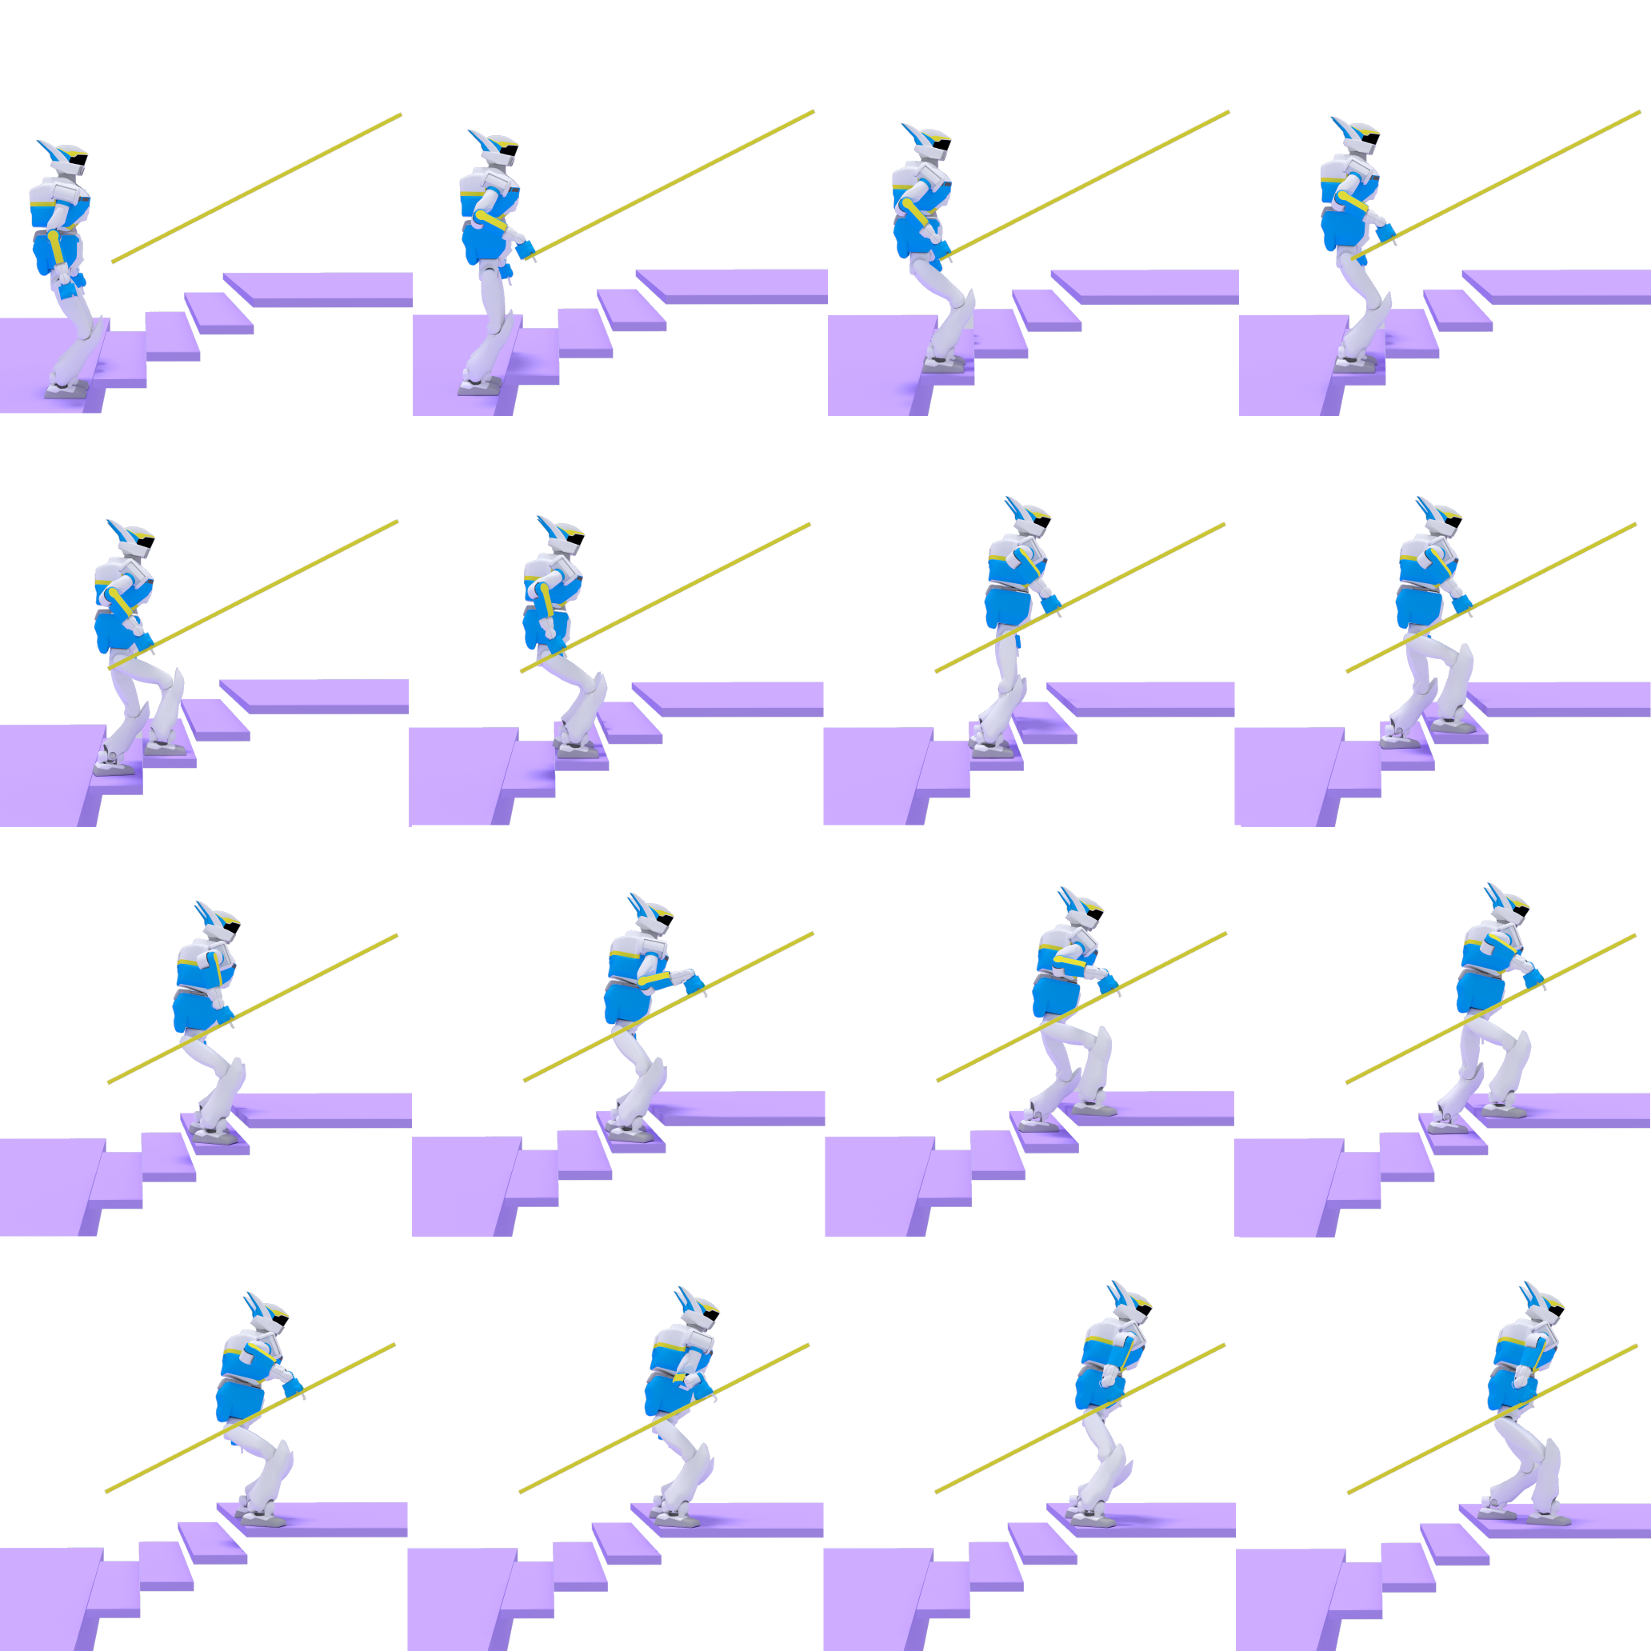
\includegraphics[width=0.5\linewidth]{figures/stair}
  \caption{
           HRP-2 in the steep stair climbing scenario. }
		   \label{fig:stair_robust}
\end{figure*}

The goal is to cross a set of stairs of a height of 20 cm. This height requires HRP-2 to use a ramp to be able to perform the task.

\noindent\textbf{Contacts involved:} Both feet and right arm.

\noindent\textbf{Heuristics:} The extended manipulability $h_w$ is chosen for the feet; $h_{EFORT}$ is chosen for the right arm.
Regarding equilibrium, the video demonstrates two sequences computed for two different treshold values of $b_0$: $0$ and $2$ (Figure~\ref{fig:stair_robust}). 

\noindent\textbf{Observations:}
This scenario illustrates best the importance of the equilibrium robustness criterion.
With a robust approach, more states are required to reach the last step (15 against 13 in average).
However, when the last step is reached by both feet, in the non robust case, the contacts are extremely close to 
the cone limits, and we believe this can be seen visually (Figure~\ref{fig:stair_comp}).


The geometry of the environment is easily addressed by our planner, and the contact planning is several times faster than real time in this scenario.

Again, the interpolation motion between the contact stances is out of the scope of this paper. However it should be noted that the computed plan in this scenario has been executed successfully on the robot~\citep{Carpentier2016}.

\begin{figure}[h!]
  \centering
  %~ 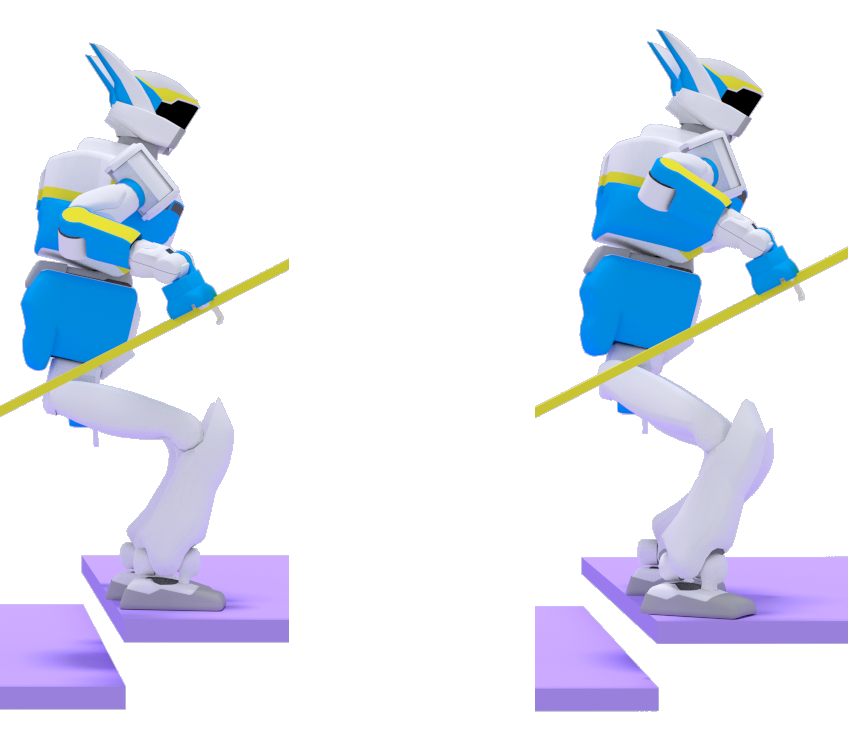
\includegraphics[width=0.6\linewidth]{figures/stair_robust}
  \begin{overpic}[width=0.5\linewidth]{figures/stair_robust}
		\put (17,5) {\small{\color{red}$b_0 = 0.23$}} 
		\put (79,5) {\small{\color{green}$b_0 = 6.16$}} 
		%~ \put (68,58) {3.a)} 
		%~ \put (5,27) {3.b)} 
		%~ \put (37,27) {4.a)} 
		%~ \put (68,27) {4.b)} 
	\end{overpic}
  \caption{
           Evaluation of the robustness $b_0$ of two contact configurations. Although in equilibrium, the left configuration is on the verge of slipping.}
		   \label{fig:stair_comp}
\end{figure}

\subsubsection{HRP-2 -- Standing up (Figure~\ref{fig:standing}):}
From a bent configuration, a standing up motion is computed in a cluttered environment.
The resulting motion involves using a wall as support, and crossing a 25 cm high stair.

\begin{figure*}
  \centering
  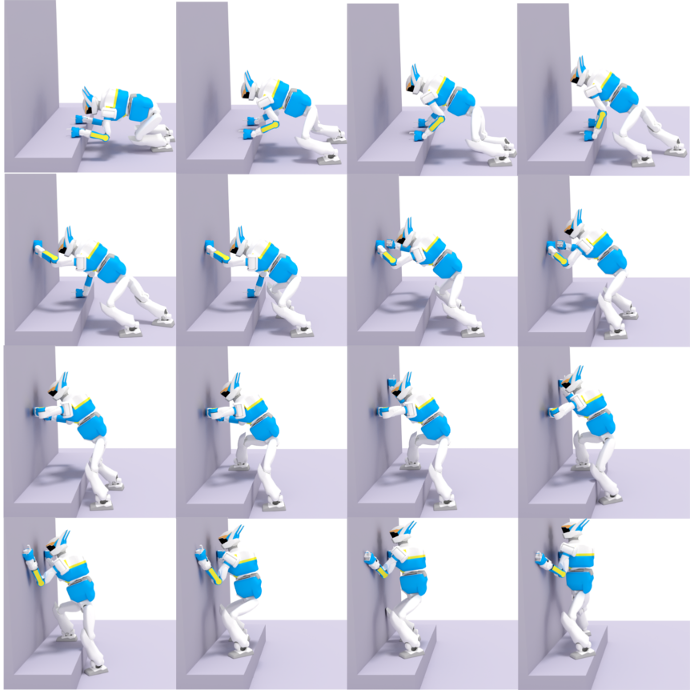
\includegraphics[width=0.5\linewidth]{figures/standing}
  \caption{
           HRP-2 in the standing scenario. }
		   \label{fig:standing}
\end{figure*}


\noindent\textbf{Contacts involved:} All (both feet and hands).

\noindent\textbf{Heuristics:} $h_w$ is used for the feet, $h_{EFORT}$ is used for the hands.

\noindent\textbf{Observations:} The scenario illustrates well the acyclic aspect of the planning. For instance, in the 4 first frames of Figure~\ref{fig:standing}, we can see that the right foot
is moved twice, with the left foot in between, before the configuration allows HRP-2 to move its hand.
Because the contacts are tried in a FIFO manner, the fact that the output contact sequence is acyclic shows that a cyclic approach (with a finite state machine for instance) is not sufficient
for the computed trajectory. The reason for this is not reachability, but equilibrium. The planning is slower than for the stair scenario (because the contact generation fails more),
though it remains compatible with interactive performances.

\subsubsection{HRP-2 -- Truck egress (Figure~\ref{fig:TODO}):}
HRP-2 stands half sitted in a truck, and is required to exit through the front window.

%~ \begin{figure*}
  %~ \centering
  %~ 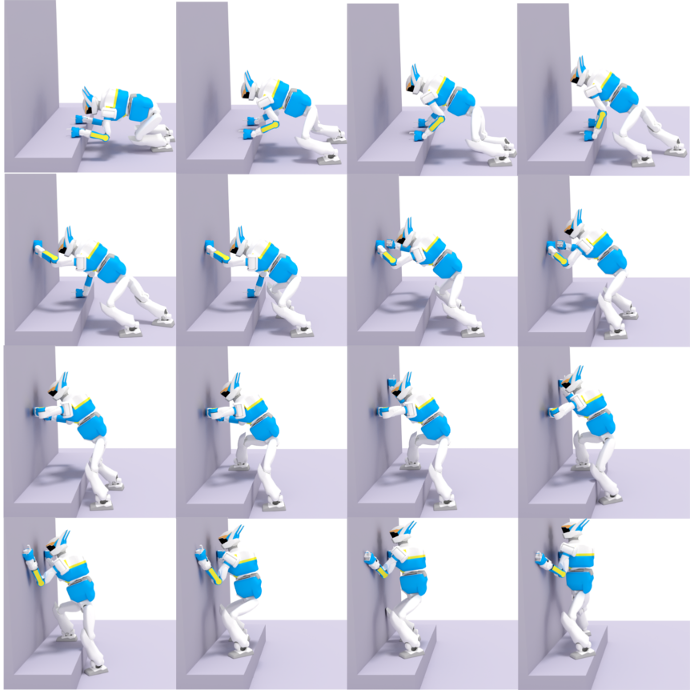
\includegraphics[width=0.5\linewidth]{figures/standing}
  %~ \caption{
           %~ HRP-2 in the standing scenario. }
		   %~ \label{fig:standing}
%~ \end{figure*}


\noindent\textbf{Contacts involved:} All (both feet and hands).

\noindent\textbf{Heuristics:} $h_w$ is used for the feet, $h_{EFORT}$ is used for the hands.

\noindent\textbf{Observations:} This scenario demonstrates the ability of the planner to compute a path in an extremely constrained environment. In this case,
the scenario is not always real time (TODO or is it ?): while the planner is often able to compute a guide path rapidly, in the worst case up to one minute can be spent
in the planning.


\subsubsection{HyQ -- Darpa style rubble (Figure~\ref{fig:darpa})}
The quadruped robot is given the task to cross a rubble composed of bricks rotated at different angles and directions.

\begin{figure*}
  \centering
  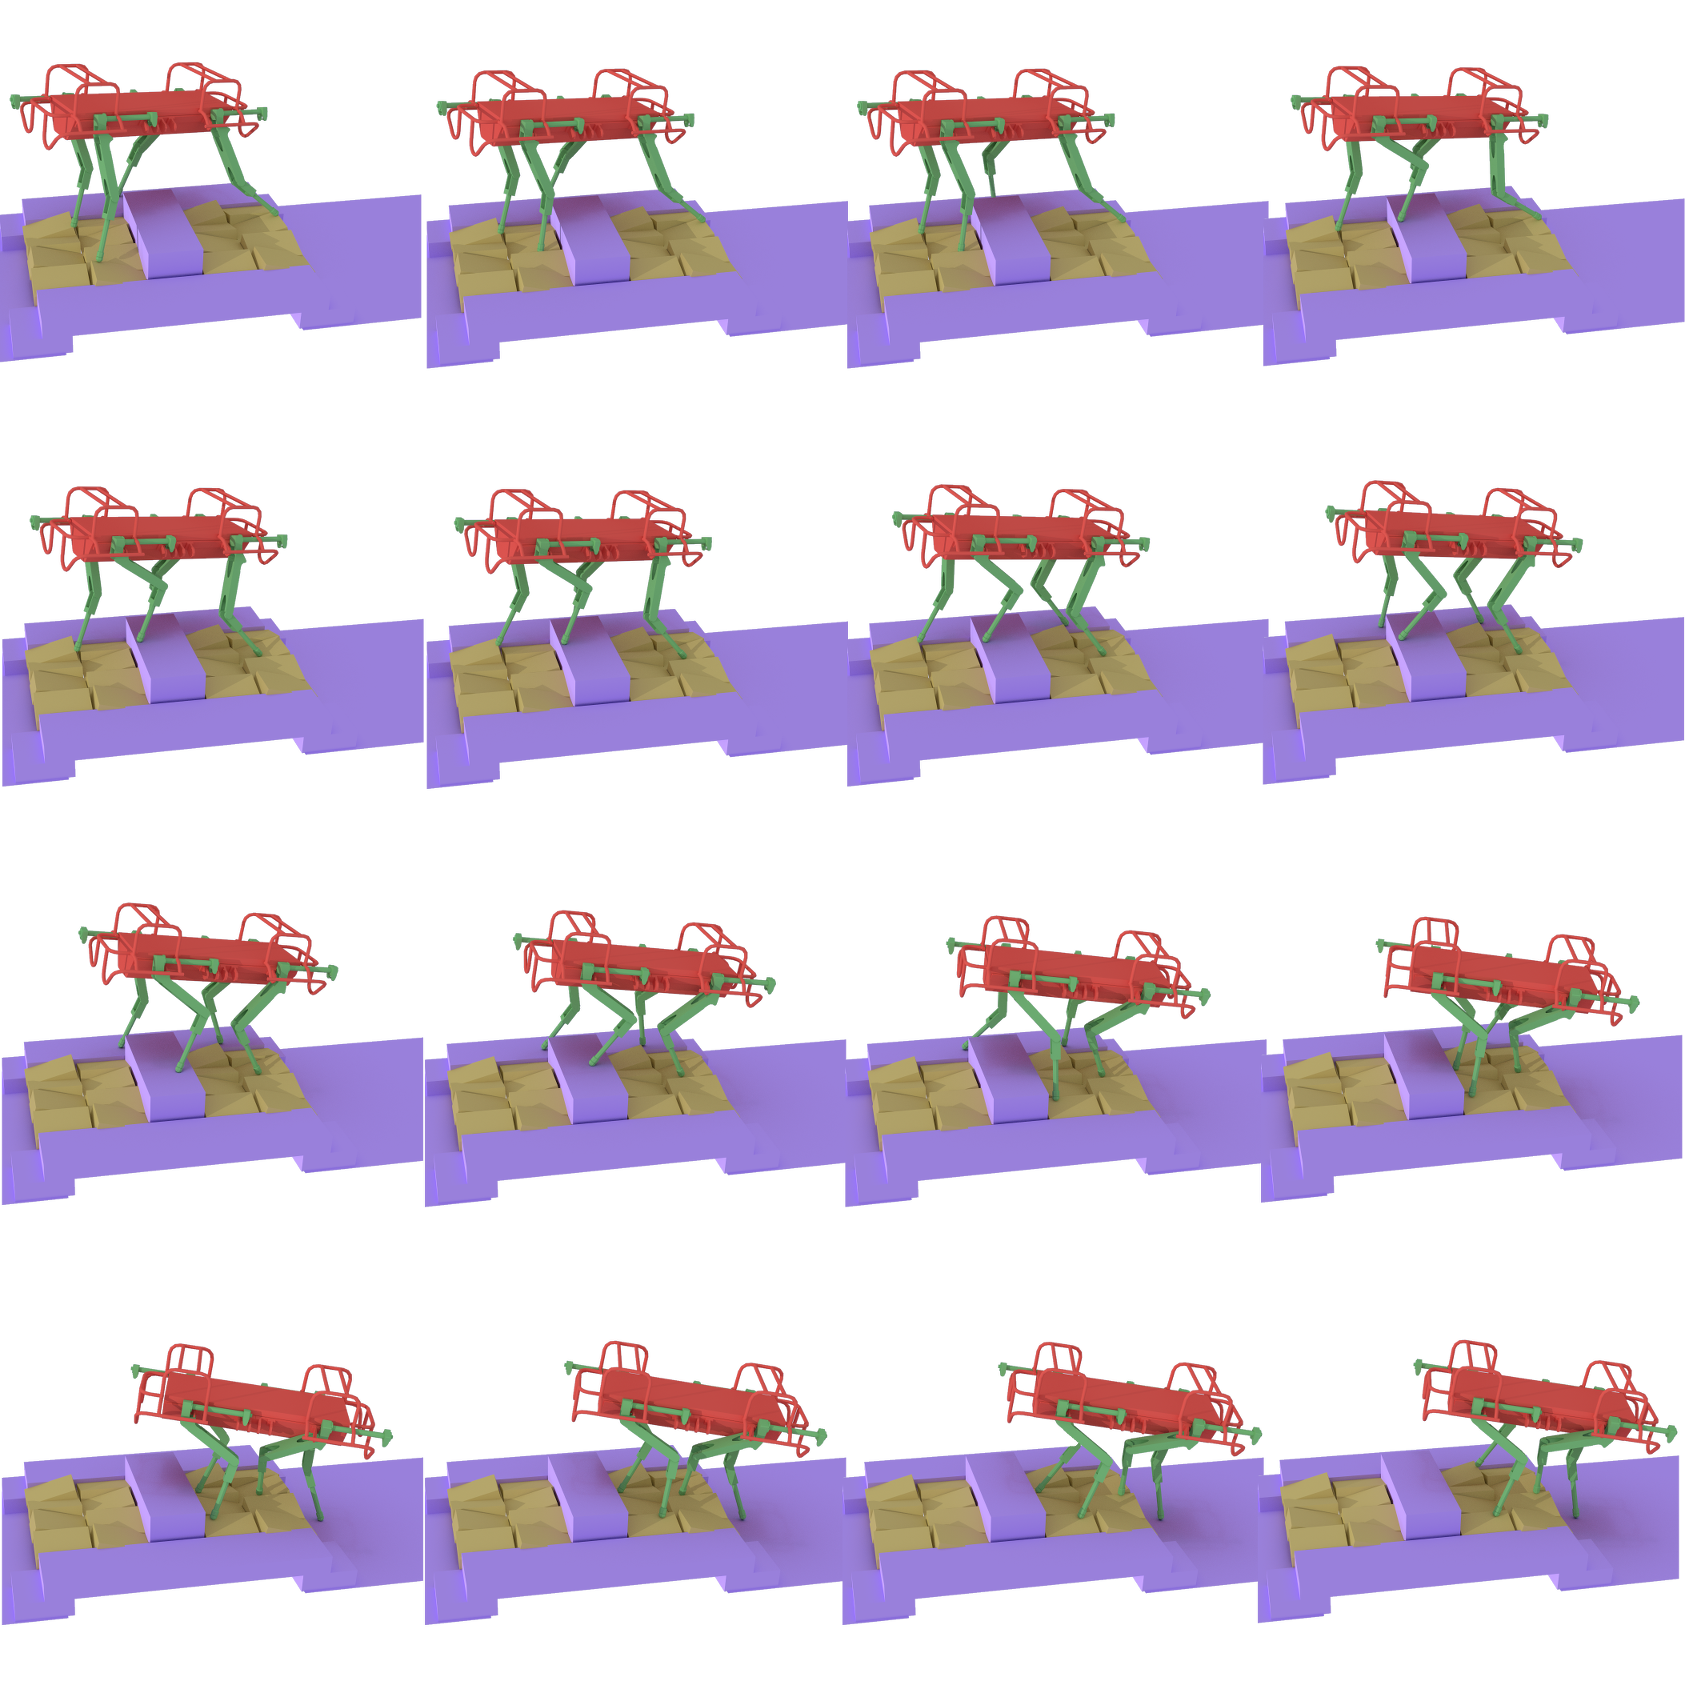
\includegraphics[width=0.5\linewidth]{figures/darpa}
  \caption{
           Robust crossing of rubbles by HyQ ($b_0 > 20$). }
		   \label{fig:darpa}
\end{figure*}


\noindent\textbf{Contacts involved:} All (the 4 legs).

\noindent\textbf{Heuristics:} $h_w$ is used for the all legs. The robustness treshold $b_0$ is set to $20$.

\noindent\textbf{Observations:} In this context, setting up a really important minimum value for $b_0$ is possible due to the high
stability of the HyQ robot, and results in more contact switches, in exchange for safety. The path planning time is higher than for the previous HRP-2 robots due to the constraint that the 4 reachable workspace of all legs must
collide with the environment at all times. Again, the computed time remains however interactive.

\subsubsection{HyQ -- Obstacle race (Figure~\ref{fig:hyq_bridge} and~\ref{fig:hyq_obs}):}
In this long scene, HyQ is first required to cross a 55 cm large hole; then, to cross a narrow "bridge", only large of 25 cm,
while maintaining equilibrium.

\begin{figure}
  \centering
  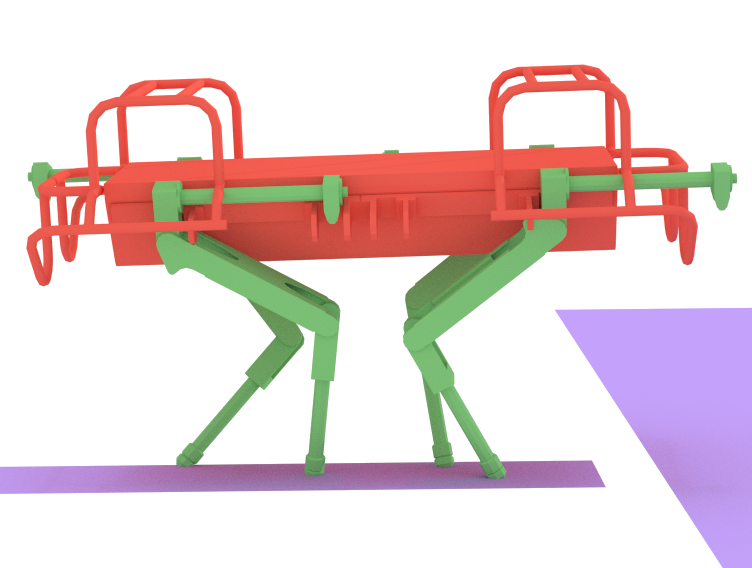
\includegraphics[width=0.4\linewidth]{figures/hyq_bridge}
  \caption{
           HyQ crossing a narrow bridge. }
		   \label{fig:hyq_bridge}
\end{figure}

\begin{figure*}
  \centering
  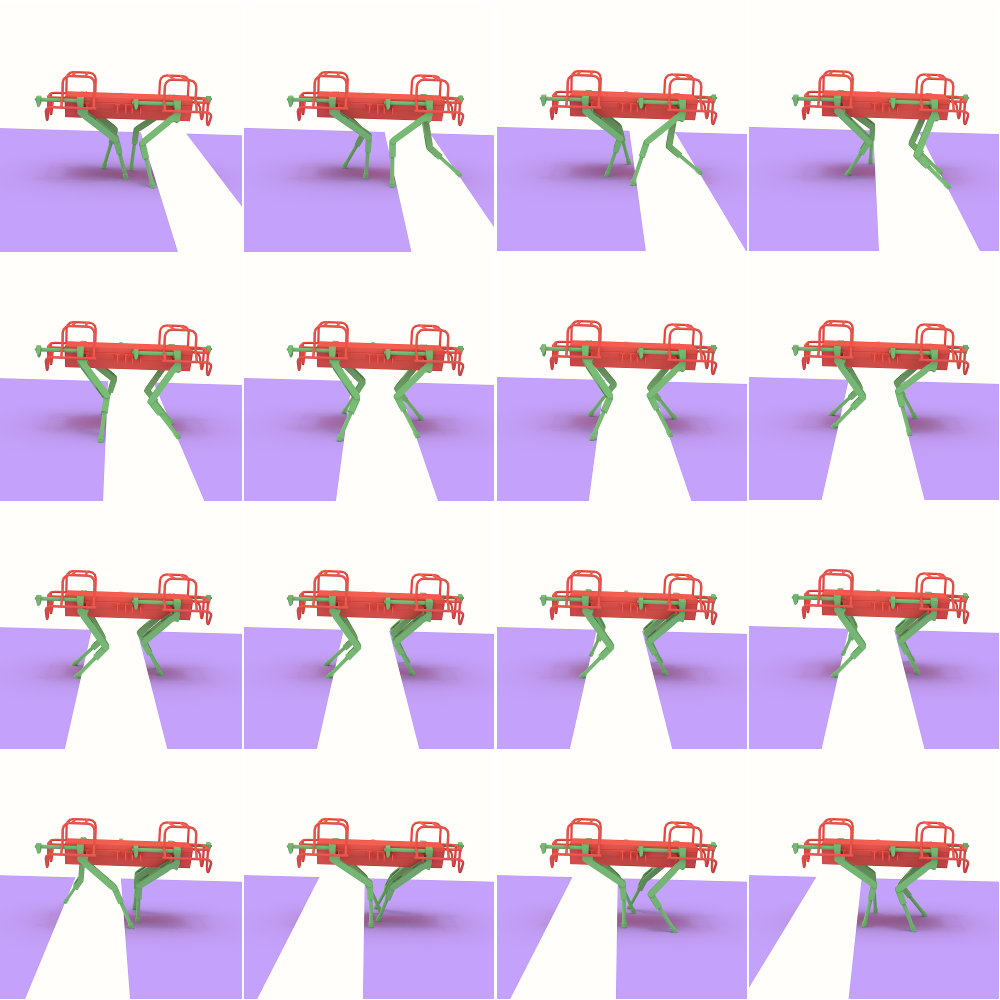
\includegraphics[width=0.5\linewidth]{figures/hyq_obs}
  \caption{
           Crossing a hole contact sequence for HyQ ($b_0 > 4$). }
		   \label{fig:hyq_obs}
\end{figure*}



\noindent\textbf{Contacts involved:} All (the 4 legs).

\noindent\textbf{Heuristics:} $h_w$ is used for the all legs. The robustness treshold $b_0$ is set to $4$.

\noindent\textbf{Observations:} Despite the apparent simplicity of the scene, this scenario is the harder to compute for our planner.
While finding a guide path above the hole is easy for the planner, finding a relevant sequence of contacts that remain in equilibrium is not trivial.
Secondly, the narrow bridge is hard both for the planner and the contact generator: To make sure that equilibrium is preserved along the traversal,
the bridge must be approached with the right angle.
This can be seen in Figure (TODO), where several feet repositionning are required to cross both obstacles (although the video shows this best).
The planner however suceeds in finding a feasible sequence in the end, again with interactive computation times.

\subsubsection{HRP-2 -- Path replanning(Figure~\ref{fig:replanning}):}
In this long scene, HRP-2 plans a path through through several obstacles. the scene is edited during the execution of the motion: a stair is added,
some stepping stones are removed, and part of the final staircase is deleted. All these modifications involve replanning.


\begin{figure}
  \centering
  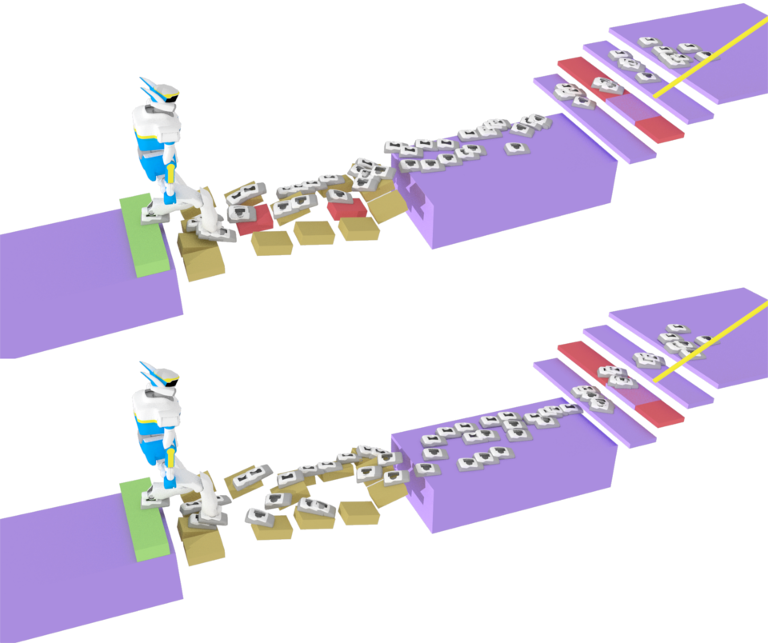
\includegraphics[width=0.7\linewidth]{figures/replanning}
  \caption{
           HRP-2 in the replanning scenario. After the red step stones are removed, a new sequence of contacts is replanned. Hand contacts
           are not presented here for readability.}
		   \label{fig:replanning}
\end{figure}

\noindent\textbf{Contacts involved:} Both feet and the right arm.

\noindent\textbf{Heuristics:} $h_w$ is used for the all legs. $h_{EFORT}$ is used for the right arm. The robustness treshold is set to $2$.

\noindent\textbf{Observations:} This scenario is designed to illustrate concretely the computation times of the planner.
In the video, the footsteps indicating the contact sequence appear at the average speed of their computation (including the guide path planning).


\subsubsection{3-fingered hand -- Manipulation of a pen (Figure~\ref{figures/penrot}):}
This scenario is proposed to illustrate the genericity of our approach: we consider a manipulation task for a robotic hand and use
our contact planner to compute a guide trajectory for the fingers, considered as effectors (Figure \ref{fig:penrot}).
Although we do not address the hard issue of accounting for rolling motions, the planner is able to compute the shown sequences, this in less than 5 seconds.

\begin{figure*}[t]
\centering
  \begin{overpic}[width=1\linewidth]{figures/penrot}
	\end{overpic}
\caption{Contact sequence found for a pen manipulation in a zero gravity environment.}
		   \label{fig:penrot}
\end{figure*}

 
\noindent\textbf{Contacts involved:} Three finger-tips.

\noindent\textbf{Heuristics:} $h_{EFORT}$ is used for the all fingers.
 
 
\subsection{Performance analysis} \label{sec:perf}
To analyze performance, for each considered scenario, we ran the simulation 1000 times.
We measured the computation time spent in each aspect of the algorithm, and also analyzed the success
rate obtained for each scenario.

Table TODO summarizes the performance measurement obtained, in terms of computation times.


\subsection{Computation times}
For each scenario, one can observe that the average computation time for one single step is largely below the second,
thus allowing to consider interactive applications. In some cases such as the stair climbing, this computation time is actually negligeable. 
Considering the repartition of the computation time, it appears that the majority of the time is spent performing inverse kinematics.
This is not surprising considering the number of calls to the methods: IK is used intensively to maintain contact continuity between two postures; 
it is also applied every time a new candidate needs to be evaluated. However regarding state of the art IK solutions, we believe there is room
for improving the performances of the algorithm.

\subsection{Success rates times}
TODO contact generation 95 %.

The other important piece of information to consider is the success rate obtained for each scenario.
With the exception of the truck egress scenario, this rate is really high.
From a pragmatic point of view, these results allow us to claim that our approach is the best current compromise between completeness and efficiency:
Indeed, the advantage of the framework is that when the contact generation fails, it does so rapidly, which allows us to replan a new contact sequence also rapidly with 
a reasonable chance of success.

\begin{table*}
\centering
\begin{tabular}{ l | >{\centering\arraybackslash}m{65pt} | >{\centering\arraybackslash}m{65pt} | >{\centering\arraybackslash}m{65pt} | c}
  &  Generate RB-PRM (offline) & Generating the contact sequence & Number of contact states\\
 \hline
   Truck egress (humanoid) & $ 73 $ & 15 & 10 \\
   Truck egress (insectoid) & $70$ & 23 & 48\\
   Climbing (humanoid)& $25$ &  5 & 15\\
   Climbing (insectoid)  & $ 21 $ & 27 & 51\\
   Crouching (humanoid)& $5$ & 6 & 22 \\
 \end{tabular}
\caption{\textbf{Average time} (in seconds) spent in RB-PRM generation, and the online generation of the contact sequence.}
\label{tab:requestime}
\quad
\end{table*}

